\documentclass{article}
\usepackage{graphicx} % Required for inserting images
\usepackage{amsmath}
\usepackage{amsthm}
\usepackage{amssymb}
\newtheorem{theorem}{Theorem}[section]
\newtheorem{proposition}{Proposition}[section]
\newtheorem{corollary}{Corollary}[proposition]
\newtheorem{lemma}{Lemma}[section]
\usepackage{nicematrix}
\usepackage{biblatex}
\usepackage{amsmath}
\usepackage{authblk}

\addbibresource{prufer_refs.bib}

\newcommand{\fzero}{\mathbf{F}_{N,0,0,k}}
\newcommand{\fm}{\mathbf{F}_{N,m,k_1,k_2}}
\newcommand{\fn}{\mathbf{F}_{N,n,k_1,k_2}}
\newcommand{\prufer}{Pr{\"u}fer }

\setlength{\hoffset}{-25pt}
\setlength{\textwidth}{400pt}

\title{Lighting up random trees: the combinatorics of partially observed transmission forests}
\author[1]{Matthew Hall}
\affil[1]{Department of Clinical Research, London School of Hygeine and Tropical Medicine, London, UK}
\date{January 2026}

\begin{document}

\maketitle

% \section{Introduction}

% The motivation behind this work is the question of what, if we can identify transmission pairs from a sample of infected hosts, we can say about the size and structure of the transmission tree or forest based on the number of pairs that we do find. Suppose:
% \begin{itemize}
%     \item $N$ is the size of a complete infected population $P$, all of which are samplable.
%     \item $n$ is the number of individuals that have been have sampled.
%     \item $k$ is the number of components of the transmission forest that are made up of the members of $P$. Each represents the descendants of a separate, independent lineage introduction to the samplable population.
%     \item $p$ is the number of pairs found.
% \end{itemize}

% We assume that we are sampling nodes from a hidden transmission $k$-forest $\mathcal{F}$ of size $N$, and that all nodes are sampled with equal probability. We also assume that if we sample two nodes then we know \emph{perfectly} whether they are adjacent in $\mathcal{T}$ (i.e. whether the hosts make up a direct transmission pair or not.) $\mathcal{T}$ is labelled with $N$ vertices numbered 1 to $N$, and without loss of generality say that the nodes are to be sampled in order of label. In the absence of any information about the tree we assume that all possible ancestries are equally likely. In this iteration no data on timings is being used, and indeed we completely ignore directionality on the first pass, so we can take $\mathcal{T}$ to be unrooted.

\section{Introduction}

The fundamental principle of genomic epidemiology is that there is a correlation between similarity between pathogen genomes and the proximity of the hosts that they were derived from in the chain of transmission. It is this principle that allows a phylogeny to be used as a proxy for a transmission tree in the field of phylodynamics, and it is this principle that allow related cases to be grouped into ``clusters'' according to a numerical threshold for genomic similarity. More recent ``source attribution'' methodologies also allow for the identification of direct transmission pairs from genomic data, often by leveraging within-host diversity.

Generally, clustering studies have been concerned solely with the investigation of individuals who are actually members of clusters, and source attribution studies the investigation of individuals who are linked another individual by transmission. This, of course, requires that other cluster members, or partners in transmission, have actually been sampled according to the protocol of the study. Both methodologies will usually also find ``singleton'' individuals whose neighbours have not been sampled, but these have rarely been the subject of investigation. Here, I suggest that this is an important omission. 

Suppose a sampling frame represents the complete set of individuals who ever could be included in a study. In our setting we assume that if an individual is sampled, they were infected with the pathogen under investigation and, moreover, the act of sampling provides a pathogen genome. The individuals making up the sampling frame are nodes in the transmission tree that represents the history of  transmissions of that pathogen, but the entire transmission tree need not be in the frame. In most cases at least some individuals have infected or been infected by members of the sampling frame will lie outside it (for example, because they live in a location where sampling was not performed). This breaks the intersection of tree and frame into \emph{forests} of those who are in both. Each component of the forest is a transmission tree, rooted at an individual whose infector was not in the frame. See figure~\ref{fig:examplett} for an example.

Suppose that a fixed number of $n$ nodes in the forest are actually sampled, and they are sampled at random. There are two properties of the forest that affect how many of the $n$ are singletons. The first is the number of components in the forest. The more of these there are, the greater the chance that two sampled individuals belong to different components. The second is just the overall number of nodes. A forest being larger will decrease the chance that two randomly-selected individuals are adjacent to each other, and thus increase the chance that any give individual is a singleton.

The distribution of singletons and non-singletons is therefore pertinent to the overall size of the samplable population, and the number of separate introductions of lineages to that population. In this paper, I explore the mathematics underlying this observation. There are three key applications of the methodology:

\begin{itemize}
    \item \textbf{Power calculations:} under assumptions about the forest, we can calculate how many samples we need to take in order to obtain a given number of linked individuals.
    \item \textbf{Hypothesis testing:} the results here are obtained under the assumption that individuals are sampled uniformly at random. This is also a fairly common assumption in clustering studies (CITE). As a particular example, sampling is assumed not to clustered and the presence of an individual in the sample does make it more likely that their direct contacts will also be in the sample. The framework here allows us to test real datasets for departure from that assumption.
    \item\textbf{Inference:} If the sampling assumptions are reasonable, this method gives a means to estimating the total size of the samplable population, and/or the number of lineage introductions to it. Neither of these is necessarily straightforward to obtain using other means. There are important caveats in doing this that we will explore later.
\end{itemize}

\begin{figure}
    \centering
    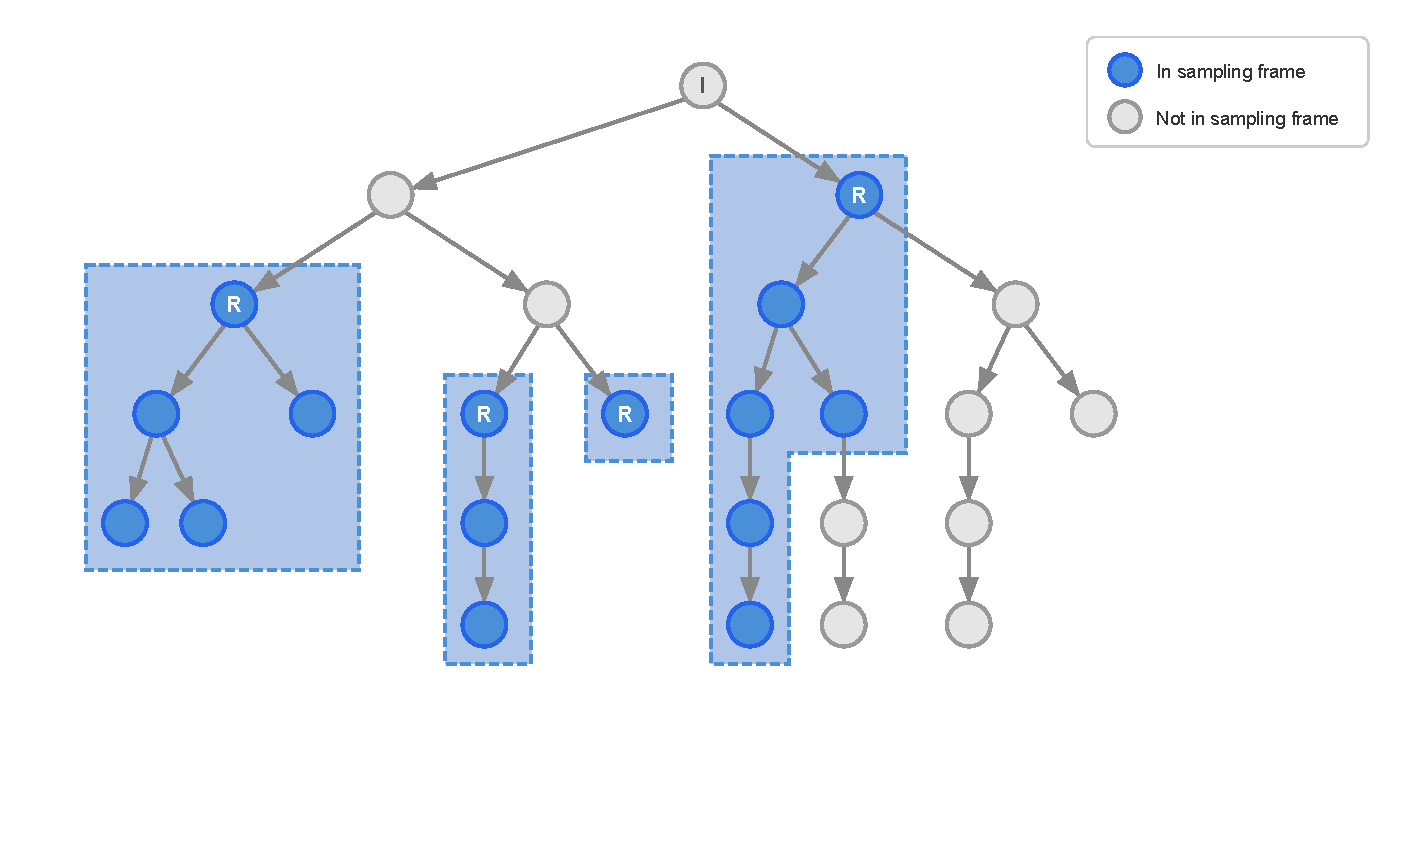
\includegraphics[width=0.9\linewidth]{transmission_tree_example.pdf}
    \caption{A full transmission tree descended from an index infection (I) but in which only 15 individuals are in the sample frame (blue). The intersection of the sampling frame with the tree produces a forest with four components, each of which has its own root node (R). On sampled individual is a singleton.}
    \label{fig:examplett}
\end{figure}

This paper starts with two mathematical sections. The first outlines the basic mathematics in detail and proves some elementary results. The second introduces a modified \prufer sequence representation of forests with the desired properties. After that, I link the previous into the epidemiological context and then show how to estimate the number of components of the forest, and the total number of trees in the forest, in a Monte Carlo sampling framework. 

\section{Labelled $k$-forests with specified independent nodes}

Let $\fzero$ be the complete set of labelled, rooted $k$-forests with $N$ nodes, where the roots are known; the labels run from 1 to $N$. The size of $\fzero$ is $kN^{N-k-1}$ \cite{Moon1970-li}. If $k_1,k_2\in\mathbb{Z}^+$ are such that $k=k_1+k_2$, let $\fn$ be the set of labelled, rooted $k$-forests such that $n$ specific nodes are independent (not adjacent to each other), and $k_1$ of the $k$ roots are amongst these $n$ while the remaining $k_2$ are not. (Note $\fm\subset\fn$ for $m>n$, and $\fzero=\mathbf{F}_{N,1,0,k}=\mathbf{F}_{N,1,1,k-1}$.) 

We will, throughout, number the $N$ nodes without loss of generality as follows:
\begin{itemize}
    \item Nodes $1$ through $k_1$ are the independent root nodes (if $k_1>0$). These are classified as ``IR''.
    \item Nodes $k_1+1$ through $n$ are the independent non-root nodes, ``IN''.
    \item Nodes $n+1$ through $n+k_2$ are the non-independent root nodes (if $k_2>0$), ``DR''.
    \item Nodes $n+k_2+1$ through $N$ are the non-independent non-root nodes, ``DN''.
\end{itemize}

\begin{proposition}\label{p1}
$|\fn|=(kN - k_1(n+k_2))N^{N-n-k_2-1}(N-n)^{n-k_1-1}$.
\end{proposition}
(Notice that this is equal to $kN^{N-k-1}$ if $n=0$ and $k_2=k$, or if  $n=1$ and either $k_2=k$ or $k_2=k-1$.) 

\begin{proof}
From the complete $N$-graph, remove all the edges connecting the first $n$ nodes, to make a graph $C^n$. The Laplacian matrix $L$ of $C^n$, with rows and columns ordered as our labels, consists of a top-left $n\times n$ block which has all diagonal entries equal to $N-n$ and 0 elsewhere, a bottom-right $(N-n)\times (N-n)$ block which has all diagonal entries equal to $N-1$ and -1 elsewhere, and all entries outside these blocks equal to -1:

\begin{align*}
L = \begin{bNiceArray}{cccc|cccc}[margin]
N-n & 0 & \cdots & 0 & \Block{4-4}<\Large>{-1}&&& \\
0 & N-n & & 0 &&&&\\
\vdots & & \ddots & \vdots &&&&\\
0 & 0 & \cdots & N-n &&&& \\
\hline
\Block{4-4}<\Large>{-1}&&&& N-1 & -1 & \cdots & -1 \\ 
&&&& -1 & N-1 &  & -1 \\
&&&& \vdots & & \ddots & \vdots \\
&&&& -1 & -1 & \cdots & N-1 \\
\CodeAfter\OverBrace[shorten,yshift=3pt]{1-1}{8-4}{n}
\CodeAfter\OverBrace[shorten,yshift=3pt]{1-5}{8-8}{N-n}
\end{bNiceArray}
\end{align*}
That the set of spanning unrooted k-forests of $C^n$ is the set of unrooted $k$-forests where the first $n$ nodes are independent should be clear after a little thought (any edges except those connecting the first $n$ nodes are permitted in members of the latter set). If $k=1$, the matrix-tree theorem \cite{Moon1970-li} states that the number of unrooted spanning trees of $C^n$ is the determinant of the reduced Laplacian, acquired by removing one row and column from $L$. 
For our purposes we want the set of spanning \emph{rooted} k-forests of $C^n$ where the roots are specified. For this we can use the All-Minors Matrix-Tree Theorem \cite{Chaiken1982-pq} which dictates that $|\fn|$ is the determinant of $L$ when the rows and columns from $1$ to $k_1$ and from $n+1$ to $n+k_2$ are removed. Call this matrix $L^{\mathrm{red}}$:

\begin{align*}
L^\mathrm{red} = \begin{bNiceArray}{cccc|cccc}[margin]
N-n & 0 & \cdots & 0 & \Block{4-4}<\Large>{-1}&&& \\
0 & N-n & & 0 &&&&\\
\vdots & & \ddots & \vdots &&&&\\
0 & 0 & \cdots & N-n &&&& \\
\hline
\Block{4-4}<\Large>{-1}&&&& N-1 & -1 & \cdots & -1 \\ 
&&&& -1 & N-1 &  & -1 \\
&&&& \vdots & & \ddots & \vdots \\
&&&& -1 & -1 & \cdots & N-1 \\
\CodeAfter\OverBrace[shorten,yshift=3pt]{1-1}{8-4}{n-k_1}
\CodeAfter\OverBrace[shorten,yshift=3pt]{1-5}{8-8}{N-n-k_2}
\end{bNiceArray}
\end{align*}
Bearing in mind the standard rules regarding elementary row operations preserving determinants, taking the first row and adding all the other rows to it gives:
\\
\begin{align*}
\mathrm{det}(L^\mathrm{red}) = 
\begin{vNiceArray}{cccc|cccc}[margin]
k_2 & k_2 & \cdots & k_2 & k & k & \cdots &  k\\
\hline
0 & N-n & & 0 & \Block{3-4}<\Large>{-1} &&&\\
\vdots & & \ddots & \vdots &&&&\\
0 & 0 & \cdots & N-n &&&& \\
\hline
\Block{4-4}<\Large>{-1}&&&& N-1 & -1 & \cdots & -1 \\ 
&&&& -1 & N-1 &  & -1 \\
&&&& \vdots & & \ddots & \vdots \\
&&&& -1 & -1 & \cdots & N-1 \\
\CodeAfter\OverBrace[shorten,yshift=3pt]{1-1}{8-4}{n-k_1}
\CodeAfter\OverBrace[shorten,yshift=3pt]{1-5}{8-8}{N-n-k_2}
\end{vNiceArray}
\end{align*}
and then by adding the first row multiplied by $\frac{1}{k_2}$ to each of the last $N-n-k_2$ rows:
\\
\begin{align*}
\mathrm{det}(L^\mathrm{red})=\begin{vNiceArray}{cccc|cccc}[margin]
k_2 & k_2 & \cdots & k_2 & k & k & \cdots &  k\\
\hline
0 & N-n & & 0 & \Block{3-4}<\Large>{-1} &&&\\
\vdots & & \ddots & \vdots &&&&\\
0 & 0 & \cdots & N-n &&&& \\
\hline
\Block{4-4}<\Large>{0}&&&& N-1+\frac{k}{k_2} & -1+\frac{k}{k_2} & \cdots & -1+\frac{k}{k_2} \\ 
&&&& -1+\frac{k}{k_2} & N-1+\frac{k}{k_2} &  & -1+\frac{k}{k_2} \\
&&&& \vdots & & \ddots & \vdots \\
&&&& -1+\frac{k}{k_2} & -1+\frac{k}{k_2} & \cdots & N-1+\frac{k}{k_2} \\
\CodeAfter\OverBrace[shorten,yshift=3pt]{1-1}{8-4}{n-k_1}
\CodeAfter\OverBrace[shorten,yshift=3pt]{1-5}{8-8}{N-n-k_2}
\end{vNiceArray}
\end{align*}
With the determinant of the bottom right block being $\frac{1}{k_2}(kN-k_1(n+k_2))N^{N-n-k_2-1}$, this is $(kN - k_1(n+k_2))N^{N-n-k_2-1}(N-n)^{n-k_1-1}$ as needed.
\end{proof}

\section{A \prufer sequence representation of $\fn$}\label{sprufer}

The standard \prufer sequence for a labelled, unrooted tree of $N$ nodes is a sequence of $N-2$ integers from $1$ to $N$. There is a bijecton between  sequences and trees \cite{Moon1970-li}. The sequence has the additional property that the degree of node $u$ in a given tree is the number of times that $u$ appears in the corresponding sequence, plus 1. The sequence is derived from the tree by sequentially removing the leaf node with the smallest label and recording the node it was adjacent to in the sequence, until only two nodes remain.

A similar construction for rooted $k$-forests can be derived by following \textcite{Lavault2011-ta}. These take the form of a sequence of length $N-k$ where the first $N-k-1$ entries are from 1 to $N$ and the last entry must be one of the $k$ roots. Construction is identical to the above except that it is the \emph{non-root} leaves with the smallest labels that are removed in turn, and that the last edge is removed and added to the sequence. (The standard construction leaves that last edge in place.) Because a $k$-forest of $N$ nodes has $N-k$ edges, removing all but one of these must leave a single leaf attached to a root, mandating that the last element in the sequence is indeed a root. The property regarding degrees is now that non-roots still appear a number of times in the sequence equal to their degrees minus 1, but roots appear a number of times equal to their degrees.

To get an intuition of the modified construction we will use in the presence of independent nodes, let $\mathbf{T}_{N,n}$ be the set of \emph{unrooted} labelled \emph{trees} with $N$ nodes, the first $n$ of which are independent. We propose a modified \prufer procedure for $\mathbf{T}_{N,n}$, taking the form of two sequences $s_1$ and $s_2$. The sequence $s_1$ is of length $n-1$ and consists only of integers from $n+1$ to $N$. The sequence $s_2$ is of length $N-n-1$ and consists of any integers from $1$ to $N$. 

If we set $k=1$ in proposition~\ref{p1}, we get that $|\mathbf{T}_{N,n}| = N^{N-n-1}(N-n)^{n-1}$, (the number of rooted trees with a specified root being equal to the number of unrooted trees). This shows that the above set of sequence pairs has the same cardinality as $\mathbf{T}_{N,n}$.

To map a tree onto such a sequence pair, we take the normal approach \cite{Moon1970-li} of repeatedly removing the leaf node with the smallest label and then recording the node it was adjacent to, until only two nodes remain. The difference is that, the first $n-1$ times we remove an independent node, we fill $s_1$. Removals of non-independent nodes fill $s_2$, as does the removal of the last independent node (if this is not one of the last pair). The entries of $s_1$ are all greater than $n$ as independent nodes cannot be adjacent to each other. One of the first $n$ nodes may be amongst the last two nodes in the tree (but two cannot be) and thus the removal of the remaining $N-n-1$ nodes may avoid it, leading in some cases to pairs of $s_1$ and $s_2$ that contain no integers between 1 and $n$.

This map from tree to sequence is injective, but this is not as plain as it is in the normal \prufer case. The proof is skipped because I prove it for the more general forest case below. As an injective map between two sets of the same size, it must be bijective. This construction also maintains the property of regular \prufer sequences in which the degree of a node is the number of times it appears in the sequence plus 1.

We now want to move to the situation of a $k$-forest. Given that there are $N-k$ edges to remove to generate the sequence, it would seem natural from proposition~\ref{p1} that we could use the same construction as above, with $s_1$ being of length $n-k_1-1$ and $s_2$ of length $N-n-k_2-1$, with there then being $kN - k_1(n+k_2)$ ways to remove the last two edges. This is, interestingly, not actually true; see figure~\ref{fig:differentnumbers}.

\begin{figure}
    \centering
    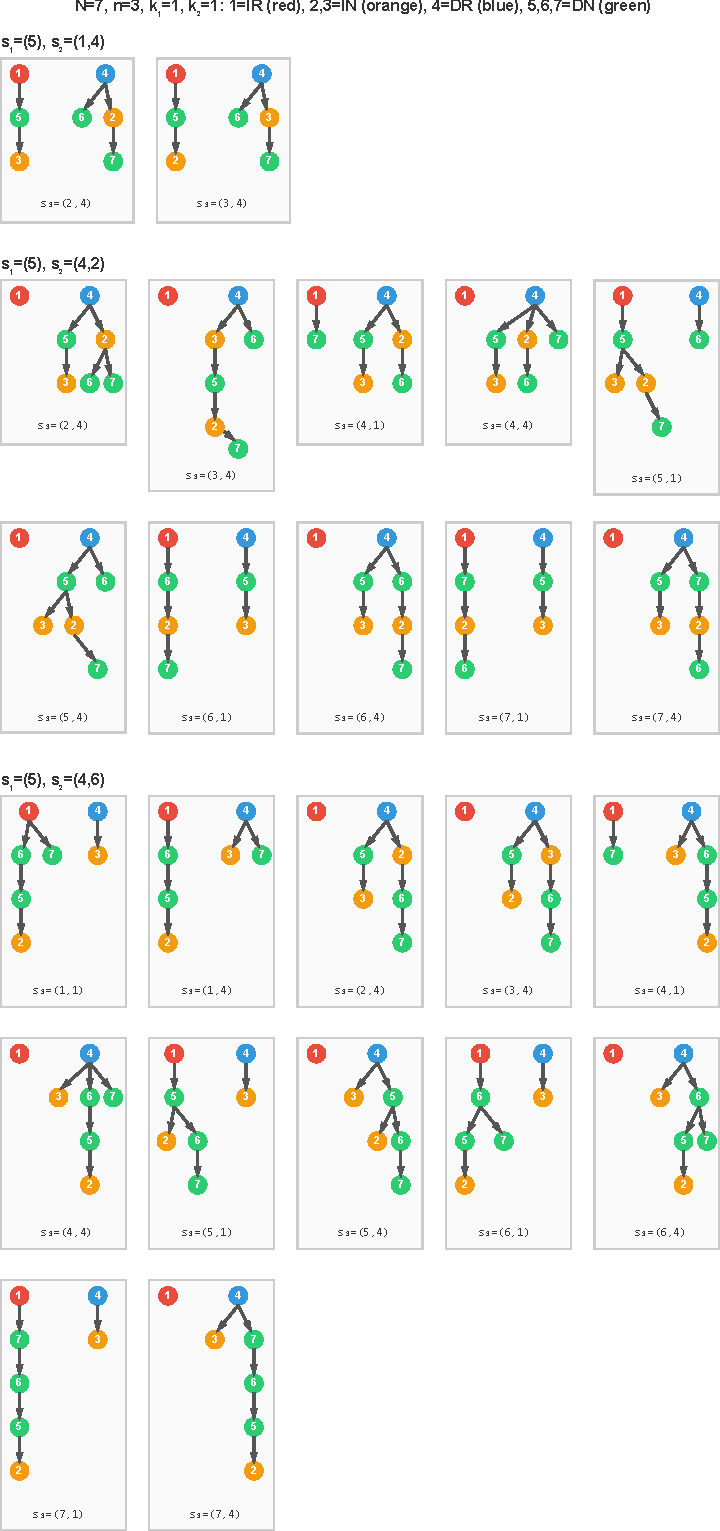
\includegraphics[width=0.58\linewidth]{24tree.pdf}
    \caption{For $N=7$, $n=3$, $k_1=1$ and $k_2=1$, different unique combinations of $s_1$ and $s_2$ have a different number of possible $s_3$s. All possible forests for three possible $s_1,s_2$ combinations are given. For $s_1=(5), s_2=(1,4)$ there are only two $s_3$s that lead to valid forests; for $s_1=(5), s_2=(4,2)$ ten, and for $s_1=(5), s_2=(4,6)$ twelve. Red nodes are IR, orange IN, blue DR, and green DN.}
    \label{fig:differentnumbers}
\end{figure}

Suppose $k_1 < n$ and $k_2 < N-n$, i.e. there exists at least one independent non-root and one non-independent non-root. (The special cases in which these are not true are considered later.) We define a triplet of sequences $s_1, s_2, s_3$ as follows:

\begin{itemize}
\item $s_1$ is of length $n-k_1-1$ and consists, if nonempty, of integers between $n+1$ and $N$.
\item $s_2$ is of length $N-n-k_2-1$ and consists, if nonempty, of integers between $1$ and $N$.
\item $s_3$ is always of length 2. Its second element is always a root.
\end{itemize}
We fill the sequences as follows:
\begin{enumerate}
    \item Select the non-root leaf node with the smallest label.
    \item If it is an independent node and there is space left in $s_1$, remove it and add the label of the node adjacent to it to $s_1$; otherwise, add it to $s_2$.
    \item Repeat the above until only two non-root nodes remain.
    \item Remove the leaf with the smaller label and add the label of the node adjacent to it to $s_3$.
    \item Remove the last leaf and add the label of the node adjacent to it (which must be a root) to $s_3$.
\end{enumerate}
We introduce two conditions on the contents of $s_2$ for what follows.
\begin{itemize}
\item\textbf{Condition 1:} $s_2$ is nonempty, the last IN in its is immediately followed by an IR, or if it has no INs, its first element is an IR.
\item\textbf{Condition 2:} The last element of $s_2$ is an IN, or $s_2$ is empty.
\end{itemize}

\begin{proposition}\label{p2}
Let $s_1\in\{n+1,...,N\}^{n-k_1-1}$ and $s_2\in\{1,...,N\}^{N-n-k_2-1}$. Suppose that we have removed the first $N-k-2$ nodes from a forest $F$ as above and and obtained $s_1$ and $s_2$. Then
\begin{enumerate}
    \item The nodes of $s_3$ are not $(\mathrm{IN}, \mathrm{IR})$ under any circumstances
    \item The nodes of $s_3$ can always be $(\mathrm{IN}, \mathrm{DR})$ regardless of the contents of $s_2$.
    \item The combinations $(\mathrm{IR}, \mathrm{DR})$ and $(\mathrm{IR}, \mathrm{IR})$ are possible if and only if neither condition 1 nor condition 2 holds.
    \item The combinations $(\mathrm{DN}, \mathrm{IR})$, $(\mathrm{DN}, \mathrm{DR})$, $(\mathrm{DR}, \mathrm{IR})$, and $(\mathrm{DR}, \mathrm{DR})$, are not possible if and only if condition 1 holds
\end{enumerate}
\end{proposition}
\begin{proof}
There are always two non-root nodes left once $s_1$ and $s_2$ are filled. If the first element of $s_3$ is IN or DN, then one is adjacent to the other, which is adjacent to a root. If the first is IR or DR, then both are adjacent to roots.

There cannot be two independent nodes left once $s_1$ and $s_2$ are filled. If there were, then they would both be pendants of DR nodes because of their independence. The removal of the third-from-last node can only then also have been the removal of of an IN, because if there was a DN present at that point, at least one of the INs would already have been a leaf and been removed  first. (IN leaves, remember, are always removed in preference to DN leaves.) The previous removal to that would also have to have been of a pendant IN, and so on until either one runs out of INs and must have removed a DN, which is a contradiction, or it turns out that there were no DNs at all, which we prohibited.

    To show 1), the above implies that the first node removed in filling $s_3$ is non-independent and adjacent to an IN, and when that is removed it would leave an IN whose removal adds an IR to $s_3$. This contradicts the definition of independence.
    
    To show 3), suppose condition 1 holds.  When the last IN is added to $s_2$, there must be at least one IN left in the forest. It is possible to then remove all but one of the remaining INs by filling $s_1$, but at that point one must enter an IR into $s_2$, which is caused by the removal of a DN. There always remains at least one IN after the IR has been placed in $s_2$, and one will remain even after $s_1$ is filled. Since INs are always removed before DNs, and it must have been the removal of a DN that added the IR to the sequence, this means that at the time the IR is added, the remaining IN is not a leaf. It also never becomes a leaf up to the point that $s_2$ is filled, because the removal of any leaf attached to it would place its number in the sequence subsequent to the IR, which we know does not happen. This means that when we have only two non-roots left, one is IN. If that IN is a leaf, then the first element of $s_3$ cannot be IR because it is added due to the removal of an independent node. If it is not a leaf, then the first element of $s_3$ is obviously IN. The logic is the same if there are no INs in $s_2$ at all; at least one must remain to be removed and it cannot be until the time comes to fill $s_3$.
    
    If condition 2 holds and $s_2$ is nonempty then there is trivially an IN left after $s_1$ and $s_2$ are filled, and the first element of $s_3$ cannot be an IR for the same reasons. So suppose it is empty. This means $N-n-k_2-1=0$, or equivalently that there is only a single DN in the forest. It is either the child of a root, or the child of an IN, and that IN must be the child of a DR. In either case it is one of the last two nodes removed and thus its removal fills $s_3$. The other removal in $s_3$ must be an IN as there are no other DNs. Hence $s_3$ cannot be (IR, IR). If both the last two nodes are children of roots, then $s_3$ cannot be (IR, DR) because the IN is removed first. 
    
    If neither condition holds, $s_2$ is nonempty and the last IN in it is followed by a DN or DR. There exist forests in which all remaining INs at that point are leaves, and they are then immediately removed, leaving only DNs left. Some of those trees also have two DNs left as leaves when $s_1$ and $s_2$ are removed, and the one of those with the smallest label is adjacent to an IR.

    For 4), we need to show that condition 1 additionally implies that the first element of $s_3$ is independent. Condition 1 implies that there is an IN in the last two nodes and we know there is always at most one. At no point in the completion of $s_1$ and $s_2$ did that node become a leaf, because it would then have been removed. This means that at the point where the last IN is entered into $s_2$, there remains at least one IN with at least one descendant DN. For the IN to last into $s_3$, that DN would have to be removed either as the last element of $s_3$, or during $s_3$ itself. The former is prohibited by condition 1 because that would make the last element of $s_2$ an IN. The latter implies that once we are down to two non-roots, the IN still has degree 2, so the first element of $s_3$ must be that IN.

    If condition 1 does not hold, then either condition 2 does, or neither does. In the former case, if $s_2$ is nonempty we have an IN at the end of $s_2$ and the last IN can have been a leaf after that. If $s_2$ is empty then (as above) there is a DN in the last two nodes and the last IN is either its child ((DN, DR) or (DN, IR)) or the child of a root and removed first ((DR, IR) or (DR, DR)). In the latter case there need be no IN in the last two non-roots, which freely allows the first element of $s_3$ to be any non-independent node.

    Both conditions 1 and 2 imply an IN in the last two non-root nodes, and there is always a forest in which that IN has degree 2 at that point and hence appears first in $s_3$. It must be followed by a DR. If the last IN in $s_2$ is followed by a DN or DR (and hence neither condition is true), then there is always a forest in which a remaining IN (of which there must be one as above) has one non-independent leaf child for each space remaining in $s_2$, and thus cannot be removed until after that is filled, but then will be as the first entry in $s_3$. This is sufficient for 2).
    \end{proof}
In figure~\ref{fig:differentnumbers}:
\begin{itemize}
    \item if $s_2=(1,4)$ then condition 1 is true, and the only possible $s_3$s are of the form (IN, DR), for which there are two options in this case.
    \item if $s_2=(4,6)$ then condition 2 is true, and $s_3$ can additionally be (DN, IR), (DN, DR), (DR, IR), or (DR, DR), which give eight more options here.
    \item if $s_2=(4,6)$ then neither condition is true, and $s_3$ can additionally be (IR, DR) or (IR, IR), giving another two options here.
\end{itemize}

    \begin{lemma}\label{l1}
    Let $l_2 = N-n-k_2-1$, the length of $s_2$, and suppose $l_2>0$. The number of $s_2$s for which condition 1 is true is $k_1N^{l_2-1}$. The number of $s_2$s for which condition 2 is true is $(n-k_1)N^{l_2-1}$. The number of $s_2$s for which neither is true is $(N-n)N^{l_2-1}$.
    \end{lemma}\label{lemmacount}

\begin{proof}
    If the first element is IR then there are $k_1$ choices for its value. The remaining $l_2-1$ positions can each take $N-n+k_1$ values. So this situation contributes $k_1(N-n+k1)^{l_2-1}$ sequences.

    Suppose the last IN is in position $i$ with $1\leq i \leq l_2-1$. The positions before $i$ can take $N$ values each; $i$ can take $n-k_1$, $i+1$ can take $k_1$, and the remaining positions $N-n+k_1$ values. The total number of $s_2$s with condition 1 is:
    \begin{align*}
    &k_1(N-n+k_1)^{l_2-1} + \sum_{i=1}^{l_2-1}N^{i-1}(n-k_1)k_1(N-n+k_1)^{l_2-1-i}\\
    ={}& k_1(N-n+k_1)^{l_2-1}\left[1+\frac{n-k_1}{N}\sum_{i=1}^{l_2-1}\left(\frac{N}{N-n+k_1}\right)^i \right]\\
    ={}& k_1(N-n+k_1)^{l_2-1}\left[1+\frac{n-k_1}{N-n+k_1}\frac{\left(\frac{N}{N-n+k_1}\right)^{l_2-1} - 1}{\frac{N}{N-n+k_1} - 1} \right]\\
    ={}& k_1\left[(N-n+k_1)^{l_2-1}+(n-k_1)\frac{N^{l_2-1} - (N-n+k_1)^{l_2-1}}{N - (N-n+k_1)} \right]\\
    ={}& k_1\left[(N-n+k_1)^{l_2-1}+(n-k_1)\frac{N^{l_2-1} - (N-n+k_1)^{l_2-1}}{n-k_1} \right]\\
    ={}& k_1N^{l_2-1}\\
    \end{align*}

    If condition 2 is true then the last entry in $s_2$ takes one of only $n-k_1$ values while the rest can take any value. The total number of $s_2$s is thus $(n-k_1)N^{l_2-1}$.
    If there are no constraints on $s_2$ then there are $N^{l_2}$ possibilities. The number where neither condition is true is thus:
    \begin{align*}
        N^{l_2} - k_1N^{l_2-1} - (n-k_1)N^{l_2-1} = (N-n)N^{l_2-1}
    \end{align*}
\end{proof}
If $l_2-0$ then there is patently only one $s_2$, for which condition 2 is true. We can now show:

\begin{theorem}\label{theorem}
Suppose $k_1 < n$, $k_2 < N-n$ and $N-n-k_2-1>0$. Let $s_1$ be a sequence of integers from $n+1$ to $N$ of length $l_1=n-k_1-1$. Let $s_2$ be a sequence of integers from 1 to $N$ of length $l_2 = N-n-k_2-1$. Let $s_3$ be a sequence of integers of length 2 whose possible contents are:
\begin{itemize}
    \item If $s2$ has condition 1, a first entry from category $\mathrm{IN}$ and a second from category $\mathrm{DR}$.
    \item If $s2$ has condition 2, a first entry from categories $\mathrm{IN}$, $\mathrm{DN}$, or $\mathrm{DR}$. If the first is $\mathrm{IN}$ then the category of the second must be $\mathrm{DR}$. If the first is $\mathrm{DN}$ or $\mathrm{DR}$, the second may be either $\mathrm{IR}$ or $\mathrm{DR}$.
    \item If $s2$ has neither condition, a first entry from 1 to $N$. If the first is $\mathrm{IN}$ then the category of the second must be $\mathrm{DR}$. Otherwise the second may be either $\mathrm{IR}$ or $\mathrm{DR}$.
\end{itemize}
The complete set of combinations of $s_1$, $s_2$, and $s_3$, $\mathbf{S}$ is in bijection with the elements of $\fn$. 
\end{theorem}
\begin{proof}
It suffices to show that the map from $\fn$ to $\mathbf{S}$ obtained by the \prufer sequence process above is injective, and that the two sets have the same size. 

For the former, suppose forests $F_1,F_2\in\fn$ are distinct. There comes a point in the process of generating the sequences where either the smallest leaves in (what remains of) $F_1$ and $F_2$ have different labels, or they do not, but the nodes they are connected to have different labels.

Suppose the former. Let $F'_1$ and $F'_2$ be the remains of the forests at this point. Suppose the smallest leaf in $F'_i$ is labelled $l_i$, and without loss of generality $l_1<l_2$. If $l_1$ and $l_2$ are leaves in both $F'_1$ and $F'_2$, then the smallest remaining leaf label in both forests is actually $l_1$, which is a contradiction. So in $F'_2$, $l_1$ is not a leaf. This implies the existence of a non-leaf, non-root node $l_3$ connected to $l_1$ in $F'_2$ where the path from $l_3$ to the root of its component passes through $l_1$. When $l_3$ is removed from forest it will add an $l_1$ to one of the sequences. But in $F'_1$, the first thing that happens is that $l_1$ is removed, thus it cannot subsequently appear in any sequence. This ensure the sequences are distinct.

So suppose the smallest leaves in $F'_1$ and $F'_2$ have the same label $l$ but are connected to nodes $p_1$ and $p_2$ with different labels. First suppose we are not filling $s_3$ at this point (i.e. $F'_1$ and $F'_2$ have at least three non-root nodes). Since whether $l$ is in the independent set is the same in both forests, this immediately causes the sequences to diverge because the next entries in $s_1$ or $s_2$ are different.

The last situation is where $F'_1$ and $F'_2$ have only one or two non-root nodes. At this point we are only filling a single sequence and the obvious injectivity of the normal \prufer construction applies.

To demonstrate that $|\fn|=|\mathbf{S}|$, suppose $\mathbf{S}_1$ is the set of combinations where $s_2$ has condition 1; $\mathbf{S}_2$ where is has condition 2, and $\mathbf{S}_3$ where it has neither.

In all cases there are $(N-n)^{l_1}$ possible $s_1$s. First suppose that $s_2$ has condition 1. By lemma~\ref{l1} there are $k_1N^{l_2-1}$ of these.  

There are then $n-k_1$ choices for the first entry of $s_3$ and $k_2$ choices for the second.
\begin{align*}
    |\mathbf{S}_1| = (N-n)^{l_1}k_1N^{l_2-1}(n-k_1)k_2
\end{align*}
If $s_2$ has condition 2, then there are $(n-k_1)N^{l_2-1}$ choices for it. Then there are $n-k_1$ choices for the first element of $s_3$ where it is $\mathrm{IN}$, and $N-n$ choices where it is not. If the first is $\mathrm{IN}$ then there are $k_2$ choices for the second. If not, then there are $k$.
\begin{align*}
    |\mathbf{S}_2| = (N-n)^{l_1}(n-k_1)N^{l_2-1}((n-k_1)k_2 + (N-n)k)
\end{align*}
If $s_2$ has neither condition, there are $(N-n)N^{l_2-1}$ possibilities. Then there are $n-k_1$ choices for the first element of $s_3$ where it is $\mathrm{IN}$, and $N-n+k_1$ choices where it is not. If the first is $\mathrm{IN}$ then there again are $k_2$ choices for the second. If not, then there are $k$.
\begin{align*}
    |\mathbf{S}_3| = (N-n)^{l_1}(N-n)N^{l_2-1}((n-k_1)k_2 + (N-n+k_1)k)
\end{align*}

Putting it all together:
\begin{equation*}
    \begin{split}
    |\mathbf{S}| ={}& |\mathbf{S}_1| + |\mathbf{S}_2| + |\mathbf{S}_3|\\
    ={}& (N-n)^{l_1}N^{l_2-1}(k_1k_2(n-k_1) + (n-k_1)^2k_2 \\&+(n-k_1)(N-n)k + (N-n)(n-k_1)k_2 \\&+ (N-n)(N-n+k_1)k) \\
    ={}& (N-n)^{l_1}N^{l_2-1}[(n-k_1)(k_1k_2 + (n-k_1)k_2 + (N-n)k + (N-n)k_2)\\&+ (N-n)(N-n+k_1)k]
    \\
    ={}& (N-n)^{l_1}N^{l_2-1}[(n-k_1)((N-n)k + Nk_2)\\&+ ((N-n)^2 + k_1(N-n))k]\\
    ={}& (N-n)^{l_1}N^{l_2-1}[n(N-n)k + (n-k_1)Nk_2 + (N-n)^2k]\\
    ={}& (N-n)^{l_1}N^{l_2-1}[kNn - kn^2 +k_2Nn - k_1k_2N +kN^2 -k2Nn +kn^2]\\
    ={}& (N-n)^{l_1}N^{l_2}[k_2n +kN -k_1k_2 -kn]\\
    ={}& (N-n)^{l_1}N^{l_2}[kN - k_1k_2 - (k-k_2)n]\\
    ={}& (N-n)^{l_1}N^{l_2}[kN - k_1(n + k_2)]
\end{split}
\end{equation*}
This is exactly the size of $\fn$ from proposition~\ref{p1}.
\end{proof}

There are three edge cases which need attention, namely when $k_1=n$ (all the independent nodes are roots) $k_2=N-n$ (all the non-independent nodes are roots), and $N-n-k_2-1=0$ (there is only one DN and $s_2$ is empty). In the former two cases $s_1$ and/or $s_2$ would have length equal to -1 and so the above construction does not work. 

The $k_1=n$ situation is actually equivalent to $n=0$; if all the independent nodes are anyway roots, it does not matter whether they are designated as independent or not. In this case the standard \prufer series representation for a $k$-forest can be used \cite{Lavault2011-ta}. If $k_2=N-n$, then the only nodes that are not roots are independent, which means they must each be a leaf attached to a non-independent root. There are $k_2$ choices for where each can be attached to, and an obvious Pr{\"u}fer-esque representation is simply a sequence of length $n-k_1$ whose elements can be from $n+1$ to $N$. If both $k_1=n$ and $k_2=N-n$ then all nodes are roots and there is trivially only one possible forest represented by an empty sequence.

If $s_2$ is empty then condition 2 is true by construction, but there is only one $s_2$ and the formula of lemma~\ref{l1} is not correct. The series has an $s_1$ (also possibly empty) of length $n-k_1-1$, and an $s_3$ whose choices are dictated by proposition~\ref{p2}; as in theorem~\ref{theorem} there are $(n-k_1)k_2 + (N-n)k$ options for the latter.

As an aside, $\mathbf{S}_1$ is the only subset of $\mathbf{S}$ that can be empty if $l_2\neq0$, and always is when $k_1=0$ or $k_2=0$. The condition on $s_2$ requires at least one $\mathrm{IR}$, and the only possible $s_3$s involve a $\mathrm{DR}$.

As before, roots appear in the combination of $s_1$, $s_2$ and $s_3$ a number of times equal to their degree, and non-roots a number of times equal to their degree minus 1.

\section{The bridge to epidemiology}

Suppose that we have a population of individuals infected by an infectious disease that we can sample from. These individuals form a transmission forest, although not necessarily a transmission tree as the individuals needed to make the graph connected may not be in the sampling frame. Also assume that, given if we have sampled two individuals, we can tell perfectly whether they make up a direct transmission pair or not (although not necessarily the direction of transmission). We want to interrogate the number of pairs that are found for a given sample size for information about the total population.

We are interested in the probability that $n$ randomly selected nodes of a fixed (but unknown) $k$-forest with $N$ nodes are independent. Lemma~\ref{l2} moves this to an easier space to work with.

\begin{lemma}\label{l2}
    The probability that $n$ randomly selected nodes of a fixed $F\in\fzero$ are independent is equal to the proportion of elements of $\fzero$ in which the nodes represented by a fixed set of $n$ labels are independent.
\end{lemma}
\begin{proof}
    Let $I(S, F)$ be an indicator function for whether the set of nodes labelled from a set $S_n\subseteq\{1,\cdots,N\}$ of size $n$ are independent in $F$. The probability that a random set of $n$ such nodes is independent is then:
    \begin{align*}
        \frac{1}{{N \choose n}} \sum_{S_n} I(S_n, F)
    \end{align*}
    and if we now ackowledge that $F$ is unknown this becomes:
        \begin{align*}
        P_1 = \frac{1}{|\fzero|}\sum_F\left(\frac{1}{{N \choose n}} \sum_{S_n} I(S_n, F)\right)
    \end{align*}
    Changing the order of summation this becomes:
    \begin{align*}
        \frac{1}{{N \choose n}}\sum_{S_n}\left(\frac{1}{|\fzero|}\sum_F  I(S_n, F)\right)
    \end{align*}
    The inner sum is the probability $P_2$ that the members of $S_n$ are independent in a random draw from the set of forests, and since labels are interchangeable this is constant. Hence $P_1 = (1/{N\choose n}){N\choose n}P_2=P_2$.
\end{proof}

The upshot of lemma~\ref{l2} is that, without loss of generality, we can assume that we have sampled nodes 1 to $n$, and the probability that those are independent across all elements of $\fzero$ is equal to the probability that a random draw of $n$ nodes of a fixed but unknown $F\in\fzero$ are independent. The former probability is the ratio of the number of elements of $\fzero$ in which the $n$ are independent to the total size of $\fzero$. The previous sections outline how to count these.

\begin{proposition}
    If the samplable transmission forest $F$ has $k$ components and $N$ nodes, then the probability of identifying no pairs in $n$ draws is
        \begin{align*}
        \frac{1}{k{N\choose k}}\sum_{k_1=0}^k {n\choose k_1}{{N-n}\choose k-k_1}(kN - k_1(n+(k-k_1)))N^{k_1-n}(N-n)^{n-k_1-1}
    \end{align*}
\end{proposition}
\begin{proof}
    If we find no pairs, then the first $n$ nodes in $F$ are independent.

    The total number of rooted $k$-forests with $N$ nodes and specified roots is $kN^{N-k-1}$ \cite{Moon1970-li}. If the roots are unknown, then there are ${N\choose k}$ ways of picking them, giving a total of ${N\choose k}kN^{N-k-1}$ forests.

    The total number of rooted $k$-forests with $N$ nodes and the first $n$ independent, where $k_1$ roots lie between 1 and $n$ and $k_2$ do not, is $(kN - k_1(n+k_2))N^{N-n-k_2-1}(N-n)^{n-k_1-1}$ by proposition~\ref{p1}. For a given $k_1$ there are ${n\choose k_1}{{N-n}\choose k_2}$ ways of picking the exact roots.

    The total number of forests where the $n$ are independent is thus:
    \begin{align*}
        \sum_{k_1=0}^k {n\choose k_1}{{N-n}\choose k-k_1}(kN - k_1(n+(k-k_1)))N^{N-n-(k-k_1)-1}(N-n)^{n-k_1-1}
    \end{align*}
    giving the result when divided by ${N\choose k}kN^{N-k-1}$.
\end{proof}

We consider situations where not every sampled individual is unlinked to all others. If we have sampled $s$ individuals, suppose the results of the genomic analysis are that they form $n$ connected subtrees each of 1 or more nodes. There are two possible situations:
\begin{itemize}
    \item In each subtree we know the exact ancestral relationship between the individuals, including which was the first infected (the root of the subtree)
    \item We know that the members of a subtree form a cluster; all are related to one of the others by direct transmission. We do not know exactly who infected who.
\end{itemize}
In either case, let $S$ be a vector of $n$ positive integers, representing the sizes of all the subtrees. We would like to be able to calculate the likelihood:
\begin{align}\label{intractable}
    L(k,N|S) = p(S|k,N)
\end{align}
This does not appear to have a closed form, and a recursive calculation quickly becomes computationally intractable, for reasons we will return to.

If we are sampling from a $k$-forest of $N$ nodes, note that all the subtrees form independent sets, in that no node from one of them is adjacent to a node from any other. The total number of nodes in all the subtrees is $n+\sum_{s\in S}(s-1)$. We can collapse each subtree to a single node to get a $k$-forest on $N'=N - \sum_{s\in S}(s-1)$ nodes in which a specified set of $n$ are independent. Let us now introduce such a collapsed forest $F$ as a latent variable in the likelihood:
\begin{align}\label{tractable}
L(k,N|S) &= \sum_F p(S|F,k,N)p(F|k,N)
\end{align}
$p(F|k,N)$ is the probability of that a forest in $\fzero$ collapses to $F$, which is the number of forests that $F$ expands to, divided by $|\fzero|$. If the $i$th component of $S$ is $s$, then there are $s^{s-1}$ rooted subtrees that collapse to a single independent node. Furthermore, if the node $i$ in F has degree $d$, there are $d$ edges incident to it which must be attached to one of the $s$ expanded nodes. If $i$ is not a root then one of those is spoken for and must connect to the subtree's root, so there are $s^{d-1}$ choices for how to attach the incident edges. If $i$ is a root then there are $s^d$. Note that the degree of $i$ is determined by the number of times it occurs in the \prufer sequence of $F$; the same as the number of times for a root, or one more for a non-root. This means that the number of subtrees must be multiplied by $s^v$ where $v$ is the number of occurances of $i$ in the sequence, regardless of whether $i$ is a root or not.
$p(S|F,k,N)$ is the probability that the data is $S$ given that the collapsed tree is $F$. If $S$ is just clusters then this is 1 or 0; $F$ will determine the contents of a cluster. If $S$ is fully resolved subtrees then only one of $s^{s-1}$ possibilities is true, so this probability is the product of $s^{1-s}$ for all $s\in S$; this cancels with the multiplicants in $p(F|k,N)$.
The reason that equation~(\ref{intractable}) is not computable in reasonable time is that one would have to sum over all possible degree distributions of the collapsed nodes, calculations which rapidly become untenable even for quite small values of $N$. Instead, we can estimate (\ref{tractable}) in either a maximum likelihood or Bayesian framework by sampling specific forests, and we can sample those just by sampling \prufer sequences, which is extremely straightforward as they are nothing more than finite sequences of integers subject to the contraints laid out in section~\ref{sprufer}.

\section{Importance sampling framework}

We cannot sample uniformly from the set of \prufer sequences of arbitrary length, so for a Bayesian inference framework we turn to importance sampling. All inference is conditioned on $n$; the number of samples taken is background information, and this means that there are a minimum of $n$ nodes in the true forest. We suppose we desire to draw $C$ transmission forests of variable size and number of components.  Then, we draw $C$ integers $U=\{u_1,\ldots,u_C\}$ from a $\mathrm{NegBinom}(\mu, s)$ distribution. The set $\{u+n-1 | u \in U\}$ is the set of forest sizes. We pick an integer $L$ to be the mean number of components in the sampling distribution, then for each $u$, we randomly sample $k-1$ from a binomial distribution with $u-1$ trials and sampling probability $L/(u-1)$. Then we sample $k_1$ (the number of sampled roots after the forest is collapsed) from a hypergeometric distribution with population size $u$, $n$ success states and $k$ draws. Finally we uniformly sample a \prufer sequence for our determined values of $N$, $n$, $k_1$ and $k_2$; this can follow the general procedure above or the special cases for $k_1=n$ or $k_2=u-n$ above. As we know the number of possible \prufer sequences om each case, we can easily calculate probability weights for importance sampling.

Priors are necessary for $N$ and $k$; $N$ here is the total size of the samplable population, not the length of the \prufer sequence as that represents the number of nodes after the data is collapsed. There are many appropriate choices of discrete distribution on the positive integers. It should be noted that the prior on $N$ retains a dependency on $n$ and thus the lower bound should formally be $n$ as there is no scope for the samplable population to be smaller than that. Likewise the very existence of a dataset implies that the minimum value of $k$ is 1.


\printbibliography

\end{document}

